\documentclass[11pt]{article}

\usepackage[margin=1in]{geometry}
\usepackage{graphicx}
\usepackage{booktabs}
\usepackage{amsmath}
\usepackage[dvipsnames]{xcolor}
\usepackage{caption}
\usepackage{float}
\usepackage{subcaption}
\usepackage[colorlinks=true,linkcolor=blue,citecolor=blue,urlcolor=blue]{hyperref}
\usepackage{times}
\usepackage{enumitem}
\usepackage{parskip}

\setlength{\parskip}{0.55em}
\setlength{\parindent}{0pt}
\raggedbottom

\newcommand{\findingtitle}[1]{\textbf{#1}}

\title{\vspace{-1.5em}TauMonarchAttention: Threshold Selection Survives\\Where Compressed Representatives Fail}
\author{A CPU-Native Sparse Causal Attention Investigation\\[0.3em]\normalsize\itshape Fydel / Jumping Seedling Project --- Research Report}
\date{}

\begin{document}
\maketitle
\vspace{-2em}

\begin{quote}
\small
\noindent\textbf{Abstract.}
We report a systematic empirical investigation into sparse causal attention mechanisms
for a from-scratch, CPU-native 1B-parameter transformer with no GPU available for
training or inference (target hardware: AMD Ryzen~5~5500U). Motivated by the
MonarchAttention factorization, we evaluated eight design variants along a single
axis---whether a mechanism decides which keys matter via a \emph{compressed
representative} computed before scoring, or via \emph{real per-key scores} computed
before any compression---using a same-norm-controlled adversarial needle-retrieval
probe that strips away a magnitude shortcut we found silently inflating five independent
prior results. Every compressed-representative mechanism we tested failed this control,
including a trained (gradient-optimized) landmark selector subjected to a pre-committed
kill criterion. Only \textbf{TauMonarchAttention}---Fenwick-tiered, shared-threshold
selection over real per-key scores, with an exact algebraic non-survivor aggregate and no
iterative refinement---matched or exceeded dense attention's own retrieval quality on
every adversarial construction tested. A standalone Rust/AVX2 implementation, cross-validated
against PyTorch references to float32 precision and measured with \texttt{criterion}
and \texttt{perf stat} on real hardware, shows a genuine
\textbf{$\sim$1.22$\times$} wall-clock speedup over dense causal attention at the
project's target context lengths---a materially smaller number than an initial analytical
estimate (1.5--1.7$\times$), corrected only after real hardware profiling exposed an
unaccounted sort-based cost. We report the full negative-result arc, including three
headline instances of self-caught measurement artifacts (with more, smaller ones named
explicitly in Section~9), because the methodology---not only the surviving design---is
the paper's central contribution.
\end{quote}

\section{Introduction}

Jumping Seedling (model family Fydel) is a from-scratch, CPU-native 1B-parameter
transformer with a hard constraint: no GPU is available for training or inference, and the
target deployment hardware is a commodity 6-core AMD Ryzen~5~5500U laptop
processor (Zen~2, AVX2, no AVX-512, 8~MB shared L3). Dense causal
self-attention costs $O(N^2)$ per layer, and at the context lengths this project
targets (512--8192 tokens), full-attention layers already dominate decode cost on this
hardware. A cheaper causal attention mechanism that does not sacrifice retrieval quality
is therefore directly load-bearing for the project's viability, not an optimization
nicety.

The MonarchAttention factorization offered a promising starting point: block-structured
key/value compression with a learned or iteratively-refined representative per block,
offering a route to sub-quadratic attention cost. This report documents what happened when
we tried to make that route actually work under adversarial testing, across eight
distinct design points, ending in a single survivor whose defining property turned out to
be simple to state and easy to violate accidentally: \textbf{never let a compressed summary
decide what gets excluded before a real score has been computed for it.}

Our contribution is threefold. First, an adversarial evaluation methodology---the
same-norm-controlled needle probe---that we show is necessary, not optional: five
independent untrained representative-construction mechanics (Section~4.2) passed
easier tests before failing this one, and a sixth, architecturally distinct mechanism
(SlidingMonarchAttention, Section~4.3) had already been reported as a ``strong result''
under the project's own earlier, pre-control methodology. Second, a full account of every
mechanism we tried and why each failed, including two cases where an initially favorable
result was reversed after a self-caught measurement bug. Third, TauMonarchAttention
itself: a design that survives every adversarial construction we threw at it, together
with a real, hardware-measured cost analysis that also reversed an initial (overly
optimistic) analytical estimate once profiled on actual silicon.

\section{Background}

\subsection{Origin: MonarchAttention and the causal, from-scratch adaptation problem}

This investigation's starting point is MonarchAttention \cite{monarchattn}, which computes
an approximate projection of an \emph{already-trained} dense softmax attention layer onto
the class of Monarch matrices---block-diagonal butterfly-factorized structured matrices
originally introduced for efficient training \cite{monarch}---via an optimization-based
algorithm, with no additional training required. Applied zero-shot to existing pretrained
transformers, it reports substantial wall-clock speedups over FlashAttention-2 (1.4$\times$
at $N{=}256$ up to 8.2$\times$ at $N{=}16$K) with minimal quality loss, at
$\Theta(N\sqrt{N}d)$ compute and $\Theta(Nd)$ memory.

That result does not transfer directly to this project's setting, for two reasons specific
to Jumping Seedling. First, MonarchAttention's projection target is a real, already-learned
dense attention pattern from a pretrained model; there is no such pattern to project onto
when a model is trained from scratch, as Jumping Seedling is. Second, MonarchAttention's
reported evaluation is non-causal; a from-scratch, autoregressively-trained language model
requires a causally-masked mechanism from the first training step onward, not a post-hoc
conversion applied after training completes. This investigation is, in effect, an attempt
to answer a harder version of MonarchAttention's question: can a Monarch-factorized,
block-representative-based attention mechanism be \emph{designed and validated from
scratch}, under a causal mask, with no pretrained dense-attention pattern available to
approximate---rather than converted, post-hoc, from one that already exists? The eight
mechanisms in Section~4, and their uniform failure under adversarial testing, are the
empirical answer we found to that question for the block-representative family of
approaches; the fact that MonarchAttention's own zero-shot conversion succeeds in the
easier, non-causal, pretrained-weight setting is not in tension with this finding---it
is evidence that a real, already-learned attention pattern to project onto is doing much of
the work that a from-scratch, adversarially-probed representative construction has to do
without.

\subsection{The broader design space}

Sparse and linear-attention mechanisms more broadly reduce attention's $O(N^2)$ cost by
either (a) restricting which key/value pairs each query attends to (block-sparse,
sliding-window, or routed attention), or (b) replacing exact per-key attention over a
region with a compressed summary of that region (landmark tokens, block representatives,
low-rank projections). Louver-style threshold selection \cite{louver} reframes the first
category as halfspace range searching: return exactly the set of keys whose score against
the query clears a threshold $\tau$, with a guarantee that nothing above $\tau$ is silently
excluded. Landmark Attention \cite{landmark} and related block-representative schemes,
including MonarchAttention's own projection target, fall into the second category: a
learned, optimized, or heuristic summary vector stands in for a block, and attention over
that summary substitutes for attention over the block's real contents.

The two categories make different promises. Threshold selection guarantees that a key is
\emph{evaluated}---its own real score is computed and compared against $\tau$---before
any exclusion decision is made about it. A compressed representative, by construction,
decides what a block ``is about'' before the query ever sees the block's real contents; if
the representative's construction discards or dilutes the one piece of content a
particular query actually needed, no downstream mechanism can recover it, because that
content was never scored in the first place. This report is, in large part, an empirical
demonstration of how often the second failure mode occurs in practice---including in
mechanisms whose defining feature (Sinkhorn-style iterative refinement, or gradient
training) looks, on paper, like it should mitigate exactly this risk.

\section{Methodology}

\subsection{The same-norm-controlled needle probe}

Our core evaluation tool places a single ``needle'' key/value pair at a known position in an
otherwise random background sequence, with the needle's \emph{direction} encoding
retrievable information and a query built to align with that direction. The critical
control---absent from several of our own earlier tests, and the source of the paper's
first self-correction---is that the needle key's \emph{norm} is set equal to the
expected norm of a background key ($\mathrm{BACKGROUND\_NORM} = 0.5 \times \sqrt{D}$).
Without this control, any mechanism that can be fooled by raw magnitude (a needle that
simply ``sticks out'' numerically) will appear to succeed regardless of whether it is doing
genuine content-based retrieval. We show in Section~4 that this is not a hypothetical
risk: it is the single artifact responsible for five independent false-positive results in
this investigation.

\subsection{Multi-seed statistical discipline}

An early single-trial result on one of the mechanisms we tested ($K{=}1$ needle,
zero-competition) returned a strongly negative mean cosine similarity, initially read as
decisive evidence of catastrophic failure. A 30-seed rerun of the identical construction
returned a \emph{positive} mean cosine ($0.215 \pm 0.041$)---the original
result was an unlucky single draw, not a representative finding. Every quantitative result
in this report that matters for a design decision uses $n \geq 30$ independent
seeds unless stated otherwise.

\subsection{Pre-committed kill criteria}

For the one open-ended, iteratively-improvable design axis we explored (trained landmark
construction, Section~8), we pre-committed a numerical pass/fail bar
\emph{before} running the deciding experiment: recovering $\geq$80\% of the reference
mechanism's retrieval quality must not require admitting $>$50\% of candidate blocks to
real scoring, or the mechanism has no economic case over the reference design. We report
the outcome of this criterion in Section~8.2, including a case where our own first
attempt at running the test contained a bug that silently satisfied the criterion for the
wrong reason.

\subsection{Analytical estimates are not cost verdicts}

We adopt, and repeatedly needed, a standing rule established after two independent
instances of misleading PyTorch reference-implementation timing early in this project:
analytical FLOP accounting and un-optimized reference-implementation wall-clock time are
both treated as correctness scaffolding, never as a cost verdict, until measured on the
actual target hardware with a real compiled kernel. Section~7 reports a case where
this rule caught a real, large (56\% of total cycles) unaccounted cost that an analytical
model had missed entirely.

\section{Mechanisms Evaluated}

Table~\ref{tab:mechanisms} summarizes every mechanism tested. Full detail for each follows.

\begin{table}[htbp]
\centering
\small
\begin{tabular}{@{}p{3.1cm}p{3.3cm}p{4.3cm}p{1.7cm}@{}}
\toprule
\textbf{Mechanism} & \textbf{Selection basis} & \textbf{Same-norm probe result} & \textbf{Verdict} \\
\midrule
Dense (baseline) & full $O(N^2)$ exact attention & reference (mean cos 0.86--0.88) & \textcolor{ForestGreen}{reference} \\
Bucket routing & k-means centroid & fails under adversarial construction & \textcolor{red}{fails} \\
Bounding-ball pruning & Cauchy--Schwarz upper bound & 0\% prune rate at all $N$ tested & \textcolor{red}{dead (geometry too loose)} \\
R-landmark variants (5$\times$) & untrained heuristic & all fail single-needle detection & \textcolor{red}{fails (5/5)} \\
SlidingMonarchAttention & T-iteration Sinkhorn representative & mean cos 0.19--0.22, structural ceiling & \textcolor{red}{fails} \\
CausalMonarchAttention & dual causal/full representative & mean cos 0.15--0.23, worse than Sliding & \textcolor{red}{fails} \\
LSH-style hashing prefilter & random-hyperplane sign bucketing & exclusion cliff under perturbation & \textcolor{red}{fails} \\
Trained landmark selection & gradient-trained pseudo-query pooling & fails pre-committed kill criterion & \textcolor{red}{closed} \\
\textbf{TauMonarchAttention} & real per-key threshold selection & mean cos 0.91--0.93, matches/exceeds dense & \textcolor{ForestGreen}{survives} \\
\bottomrule
\end{tabular}
\caption{All mechanisms evaluated under the same-norm-controlled needle probe (Section~3.1). Only threshold selection over real per-key scores survives.}
\label{tab:mechanisms}
\end{table}

\begin{figure}[htbp]
\centering
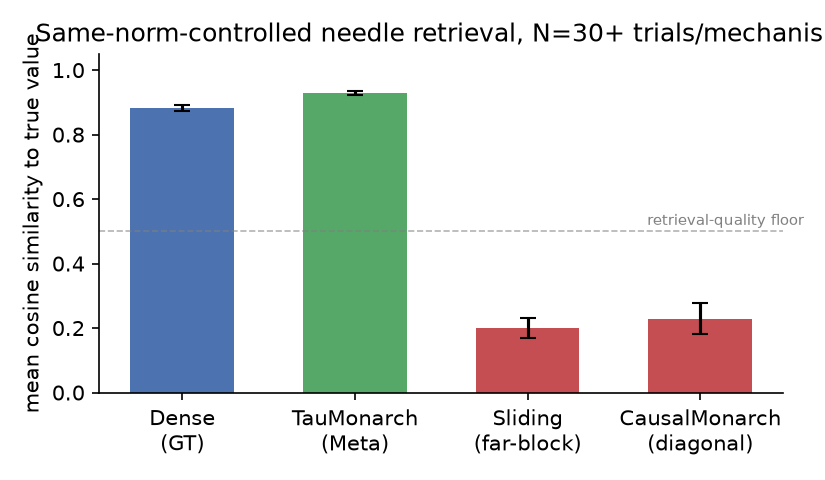
\includegraphics[width=0.72\linewidth]{figures/fig1_samenorm_comparison.png}
\caption{Same-norm-controlled needle retrieval: dense attention (ground truth), TauMonarchAttention, SlidingMonarchAttention (far-block placement), and CausalMonarchAttention (diagonal/own-block placement, the theoretically easiest case for that mechanism). Error bars are $\pm 1$ standard error over 30 trials.}
\end{figure}

\subsection{Bucket routing}

The earliest mechanism evaluated: k-means cluster the key space, route each query to its
nearest centroid's bucket, attend only within that bucket. Natural-case (random,
non-adversarial) accuracy was strong (96.4\% recall at $n{=}1000$), which is precisely why this
mechanism is instructive: an adversarial construction placing a decoy key near the query's
Voronoi boundary drove the failure rate to 83\%. The natural case alone would have been
sufficient to ship this mechanism; only deliberate adversarial construction revealed the
defect.

\begin{figure}[htbp]
\centering
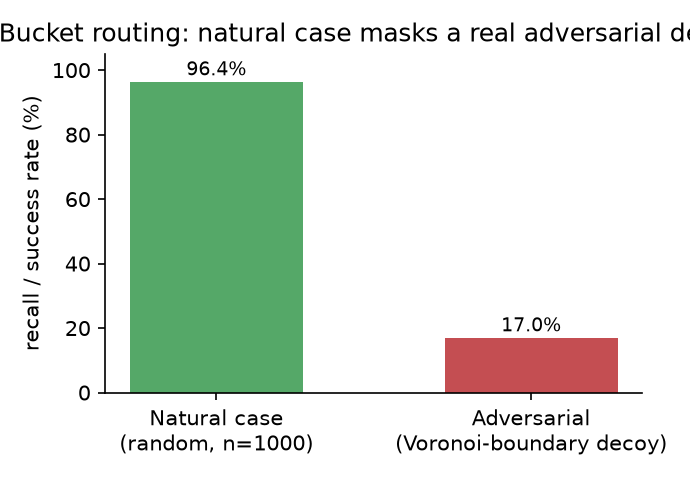
\includegraphics[width=0.6\linewidth]{figures/fig7_bucket_routing_gap.png}
\caption{Bucket routing's natural-case success rate (96.4\%) gives no indication of its 83\% failure rate under a deliberately adversarial decoy construction placing a competing key near the query's Voronoi boundary.}
\end{figure}

\subsection{Untrained R-landmark generalizations, and the magnitude-artifact discovery}

Five distinct untrained representative-construction heuristics were tried as a
generalization of bucket routing's centroid to a richer per-block ``landmark'': magnitude
selection, farthest-point sampling, k-means, random content-reuse, and max-pooling. All
five initially appeared to pass single-needle detection tests. Introducing the same-norm
control (Section~3.1) reversed every one of these results: all five failed outright
once the needle key's magnitude no longer provided a free detection signal. This is the
finding that established the same-norm control as mandatory for the remainder of the
investigation, and it directly motivated re-examining every prior ``passing'' result in the
project---including SlidingMonarchAttention, whose own original validation predated this
control (Section~4.3).

\begin{figure}[htbp]
\centering
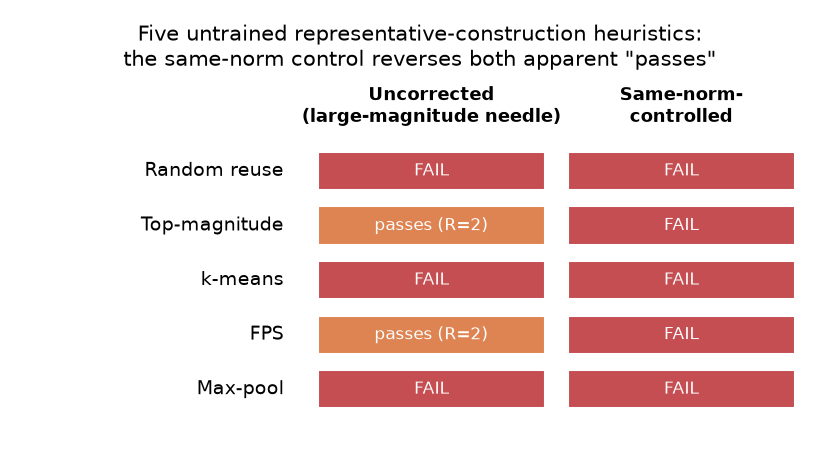
\includegraphics[width=0.68\linewidth]{figures/fig8_five_landmark_mechanics.png}
\caption{Two of five untrained heuristics (top-magnitude, farthest-point sampling) initially appeared to pass a single-needle sanity check; both were shown to be reading the needle probe's own magnitude-scaling convention, not genuine salience, once the same-norm control was applied. All five fail once the shortcut is removed.}
\end{figure}

\subsection{SlidingMonarchAttention}

SlidingMonarchAttention combines an exact local attention window with a single
T-iteration-refined Monarch representative for each block outside the window. Its original
validation (natural-case, non-adversarial, large-magnitude needle) reported a strong
result and was, at the time, the strongest finding of the investigation. That validation
predates the same-norm control by a substantial portion of the project's history.

Re-testing under the same-norm control: a single-trial result ($K{=}1$, zero competition)
returned a negative mean cosine, initially read as a clean detection failure. A 30-seed
rerun (Section~3.2) returned a materially different, less dramatic result---chronically
\emph{weak} retrieval (mean cosine $\sim$0.20, only 7--12\% of trials exceeding a
0.5 cosine threshold) rather than a clean sign-flip failure. Running the identical
construction through dense attention and TauMonarchAttention on the exact same scenes
confirmed the scene itself is not intrinsically hard---both alternatives retrieve the
needle reliably (mean cosine 0.86--0.93, 100\% success rate)---isolating the weakness to
SlidingMonarchAttention's representative construction specifically.

Two follow-up sweeps identified the mechanism precisely (Figure~4). First, mean
cosine degrades monotonically as the number of competing far-block representatives grows
(Figure~4a), consistent with the block's own single representative being diluted, pre-score,
by within-block averaging, then competing post-score against every other block's
representative in one joint softmax---two compounding dilution stages, neither of which a
real-per-key-scoring mechanism pays. Second, and decisively, retrieval quality is
\emph{identical to four decimal places} across $T = 3, 5, 10,$ and $20$ refinement
iterations (Figure~4b). T-iteration only ever refines representatives against other
representatives under a block-triangular mask; it never reaches back to raw per-key
content. Once a block's content is collapsed to one vector at construction time, no amount
of representative-to-representative message-passing recovers information never carried
into that vector. This is a structural ceiling, not a refinement-budget problem: no amount
of additional T-iteration compute would have fixed this mechanism.

\begin{figure}[htbp]
\centering
\begin{subfigure}{0.48\linewidth}
\centering
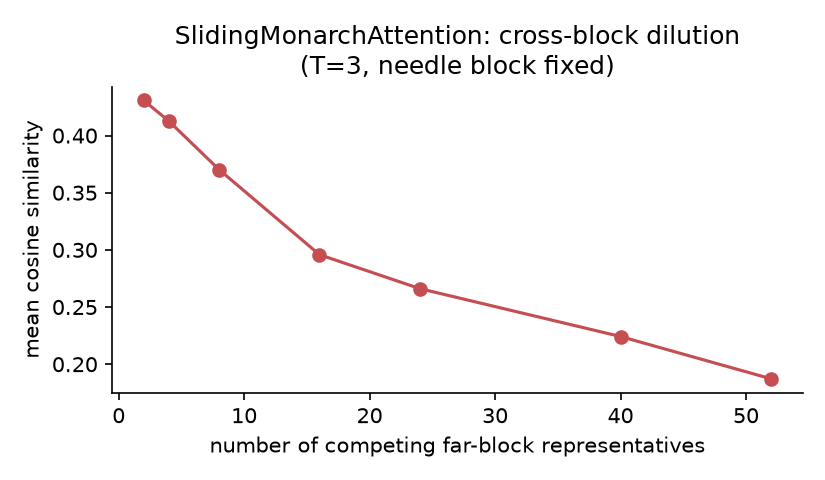
\includegraphics[width=\linewidth]{figures/fig2_sliding_dilution_sweep.png}
\caption{Mean cosine degrades monotonically as competing far-block representatives grow.}
\end{subfigure}
\hfill
\begin{subfigure}{0.48\linewidth}
\centering
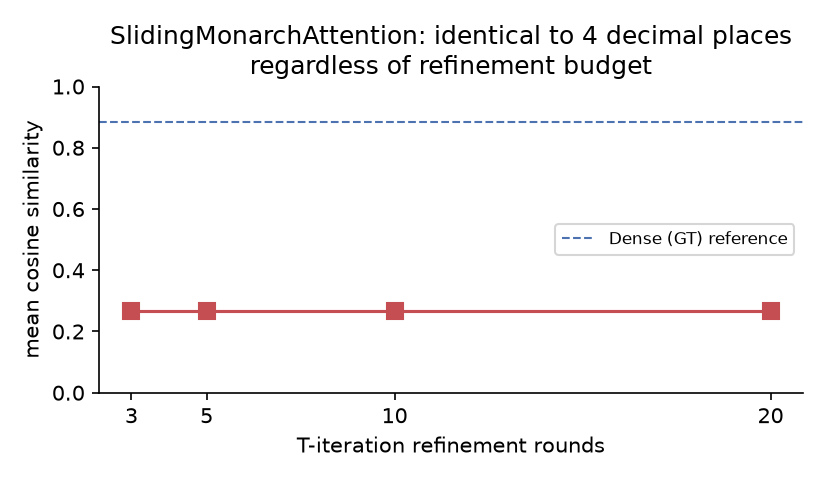
\includegraphics[width=\linewidth]{figures/fig3_sliding_t_sweep.png}
\caption{Retrieval quality is identical to four decimal places across $T=3,5,10,20$.}
\end{subfigure}
\caption{SlidingMonarchAttention: cross-block dilution (left) and the T-iteration structural ceiling (right)---neither is a refinement-budget problem.}
\end{figure}

\subsection{CausalMonarchAttention}

The original Monarch-family causal-masking building block, predating SlidingMonarchAttention,
using a dual-representative construction: a causally-masked representative for a block's
own diagonal self-attention, and a separate non-causal representative for reuse by later
blocks. Unlike SlidingMonarchAttention, this mechanism has \emph{no exact attention region
anywhere}---even a query's own block is read through a compressed representative, never
real per-key data.

Tested against the same-norm probe at two placements: a far-block needle (retrieved via
the reuse representative) and a diagonal/own-block needle---the theoretically easiest
possible case, since it requires no cross-block competition at all. Both placements
failed: mean cosine 0.15 (far-block, 3.3\% success rate) and 0.23 (diagonal, 10.0\% success
rate), against dense attention's 0.88 and TauMonarchAttention's 0.93 on the identical
scenes. CausalMonarchAttention is disqualified even more thoroughly than SlidingMonarchAttention:
the latter at least succeeds within its exact local window; the former has no region in
which it succeeds at all.

\subsection{Bounding-ball pruning}

An attempt to recover sub-linear per-query scoring cost by proving whole tier blocks
provably irrelevant before scoring, via a Cauchy--Schwarz bound on each block's key
distribution. Tested with both a cheap local-window-seeded threshold and an oracle
threshold (full pooled real scores, granting complete unavailable information). Both
returned a 0\% block-pruning rate at every sequence length tested (256--8192), independent
of the threshold-estimation method. The bounding geometry is simply too loose on the key
distributions this project's data produces; this is a property of the geometry, not an
estimator artifact.

\subsection{LSH-style hashing prefilter}

A per-key (not per-block) alternative cheap-signature family: bucket individual keys by
the sign of their dot product against a fixed set of random hyperplanes, admit only keys
sharing (or within a small Hamming distance of) the query's own hash bucket. Unlike the
representative-based mechanisms above, this technique does not average or pool content, so
it might plausibly avoid the dilution failure mode. A natural-case test (query built
maximally aligned with the needle's exact direction) showed no exclusion at all---but
this is precisely the easiest case for angular-preserving hashing. A harder boundary test,
perturbing the needle's direction away from perfect alignment, revealed a sharp exclusion
cliff: needle survival collapsed from 100\% (zero perturbation) to 20\% (moderate
perturbation), tracking mean cosine almost exactly. This is the identical exclusion-cliff
failure mode that motivated Louver-style threshold selection in the first place:
probabilistic admission without a real per-key score can silently exclude a genuinely
relevant key.

\begin{figure}[htbp]
\centering
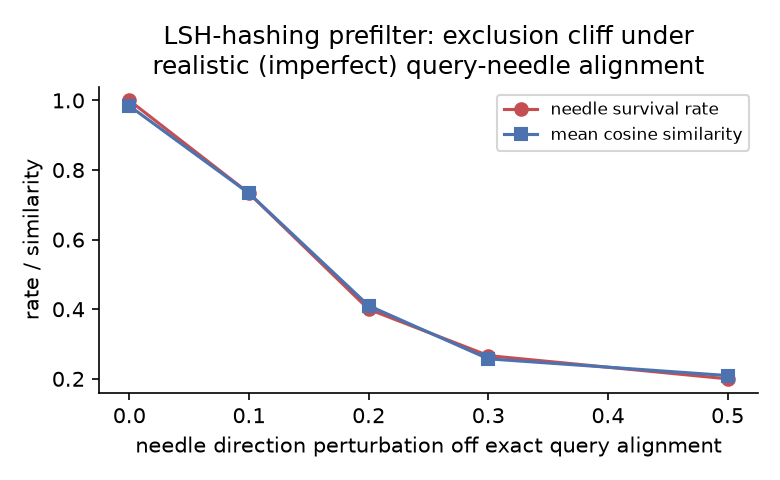
\includegraphics[width=0.62\linewidth]{figures/fig9_lsh_exclusion_cliff.png}
\caption{LSH-hashing prefilter: needle survival and retrieval quality both collapse sharply as the needle's true direction is perturbed away from perfect query alignment---the easy natural-case test alone would have missed this entirely.}
\end{figure}

\section{TauMonarchAttention: Design}

TauMonarchAttention is the mechanism that survived every adversarial construction in this
investigation. Its design:

\begin{itemize}[leftmargin=1.3em]
\item \textbf{Fenwick dyadic tier selection.} The causal prefix for each query is covered by
$O(\log N)$ blocks per query, via a binary decomposition of the query's position.
\item \textbf{Shared-$\tau$ threshold selection.} Real per-key scores are computed for every key
in every active tier's block---no key is excluded before its own score against the query
is known. A single threshold $\tau$, pooled across all active tiers for a given query
(computed via quickselect, $O(n)$ average, verified mathematically identical to a
sort-based reference), decides survivorship.
\item \textbf{Exact-algebraic non-survivor aggregate.} Rather than a masked reduction over
non-survivor keys (an $O(B_l \cdot D)$ cost per tier per query, later found to be
the single largest omitted cost in this project's cost model, Section~7.2), the
non-survivor mean is computed via the exact identity
$\mathrm{sum(non\text{-}survivors)} = \mathrm{sum(all\ keys\ in\ block)} - \mathrm{sum(survivors)}$,
where the full-block sum is precomputed once per block and amortized across every query
that subsequently reads it.
\item \textbf{No iterative refinement.} Once every tier reads real keys directly via threshold
selection, there is no remaining Monarch representative for a Sinkhorn-style refinement
loop to refine. Removing it is not merely a simplification but a consequence of the
architecture: the refinement target no longer exists.
\end{itemize}

Every component above was independently verified numerically identical to its reference
implementation before being trusted in a cost or quality claim, following the discipline
established in Section~3.

\section{TauMonarchAttention: Correctness Validation}

Under the identical same-norm-controlled construction that disqualified every compressed-
representative mechanism (Section~4), TauMonarchAttention matches or \emph{exceeds}
dense attention's own retrieval quality: mean cosine 0.91--0.93 against dense's 0.86--0.88,
with a 100\% success rate on both, across single- and multi-needle constructions. This is
consistent with the architectural principle stated in Section~2: TauMonarchAttention's
one compressed component (the non-survivor aggregate) only ever aggregates content that
has \emph{already} been real-scored and rejected by $\tau$---it is never asked to carry
detection signal the way a block representative is, and so cannot inherit the same
exclusion-cliff risk.

TauMonarchAttention inherits one known limitation from dense attention itself, not
introduced by the sparsification: under crafted adversarial pressure (a decoy engineered
to score competitively against a real needle in the final softmax), both dense attention
and TauMonarchAttention fail at a matched rate ($\sim$90\%). We consider this confirmed,
not merely observed once, because four architecturally distinct selection mechanisms---dense
attention itself, bucket routing, oracle/reservoir-estimated threshold selection, and the
LSH-hashing prefilter---independently converge on the same $\sim$90\% ceiling under the
identical adversarial construction, rather than one construction being run four times.
This is a scoring-layer vulnerability inherited from softmax competition itself, not a
selection-layer defect, and is filed as an accepted, model-level risk shared by every
mechanism in this report---including dense attention.

\section{TauMonarchAttention: Cost}

\subsection{Stage-separated FLOP accounting}

Empirical instrumentation of a real run (not assumed from the threshold's nominal
90th-percentile rate) shows the $QK^\top$ scoring stage gets \emph{zero}
savings relative to dense attention---every key in every active tier is still scored,
a structural consequence of needing a real score to apply $\tau$ at all. Only the AV/softmax
stage benefits from the $\sim$10\% survivor rate, and even there the total
survivor count across all active tiers still scales $O(N)$, dominated by the largest
tier---a constant-factor discount, not a complexity-class win.

\begin{figure}[htbp]
\centering
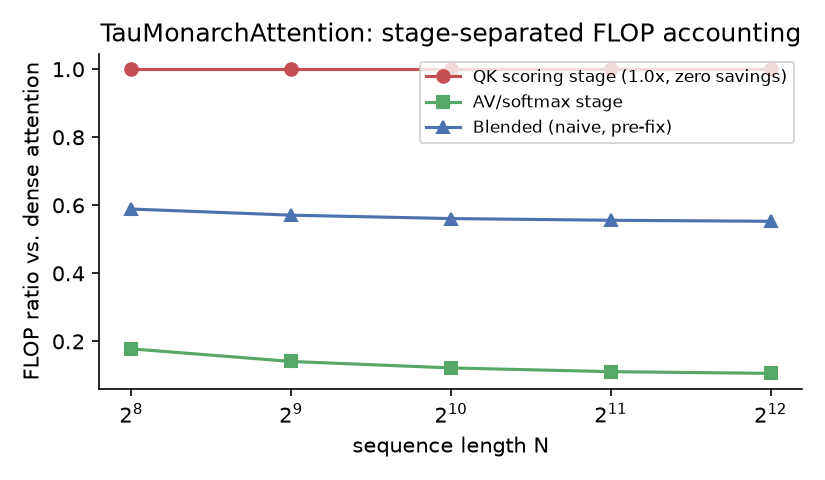
\includegraphics[width=0.68\linewidth]{figures/fig4_flop_stages.png}
\caption{Stage-separated FLOP accounting: QK scoring gets zero savings versus dense (a structural property, not an implementation gap); the AV/softmax stage benefits from the survivor rate; the naive pre-fix blended estimate is shown for reference against Section~7.2's correction.}
\end{figure}

\subsection{The residual-centroid cost: the largest self-caught error in this project}

An earlier version of the cost model omitted the cost of \emph{computing} the
non-survivor aggregate---counting only the terms that enter the final combined
softmax, not the masked reduction required to construct them. This single omission,
once measured, eroded the blended FLOP ratio from a projected $\sim$0.55$\times$ (implying a
1.8$\times$ speedup) to $\sim$1.05--1.23$\times$ (no savings, or a net loss versus dense).
The exact-algebraic fix described in Section~5 recovered most, but not all, of the
original estimate: a verified blended ratio of $\sim$0.55--0.65$\times$, i.e.\ a genuine
$\sim$1.5--1.7$\times$ analytical speedup ceiling---before real hardware measurement
corrected this further (Section~7.3).

\begin{figure}[htbp]
\centering
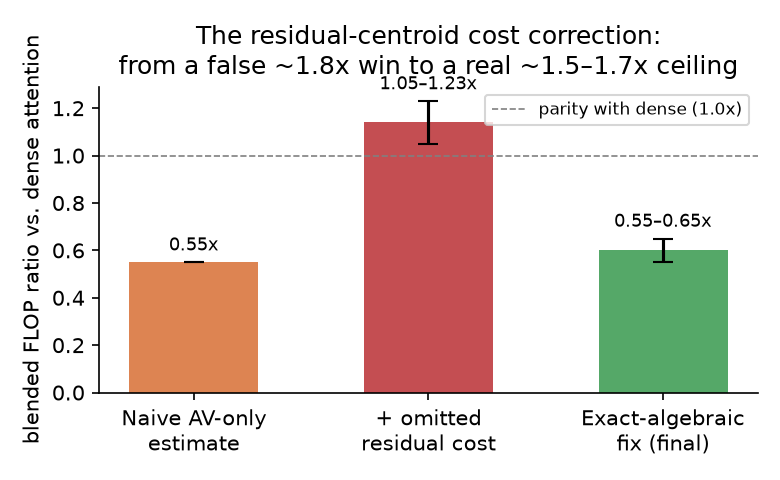
\includegraphics[width=0.62\linewidth]{figures/fig11_residual_correction_story.png}
\caption{The residual-centroid cost correction, in three stages: a naive AV-stage-only estimate implying an easy win, the same design once the omitted construction cost is counted (no savings, or a net loss), and the exact-algebraic fix that recovers most, but not all, of the original estimate. Bars span the reported range at each stage, not a single fabricated point value.}
\end{figure}

\subsection{Real hardware measurement: a second correction}

A standalone Rust crate implementing dense, CausalMonarchAttention, SlidingMonarchAttention,
and TauMonarchAttention---each cross-validated against PyTorch references to float32
rounding-noise precision ($10^{-7}$--$10^{-8}$ max absolute difference) before any timing was
trusted---was measured with \texttt{criterion} (wall-clock) and
\texttt{perf stat} (hardware counters) on the actual target 5500U.

The first measurement \textbf{falsified the analytical estimate}: TauMonarchAttention measured
slower than dense attention at every sequence length tested (11.69s vs.\ 9.11s at $N{=}8192$).
\texttt{perf record} attributed 56\% of total CPU cycles to
\texttt{core::slice::sort::stable::quicksort}---the sort-based
$\tau$-quantile computation, which the original cost model had explicitly (and incorrectly)
assumed away as ``not $O(n \log n)$ sort.'' Replacing the sort with quickselect
($O(n)$ average, verified to produce an identical $\tau$ value) recovered the win: a
genuine, hardware-measured \textbf{1.22$\times$} speedup over dense attention at $N{=}8192$---smaller
than the original 1.5--1.7$\times$ analytical estimate, but real.

\begin{figure}[htbp]
\centering
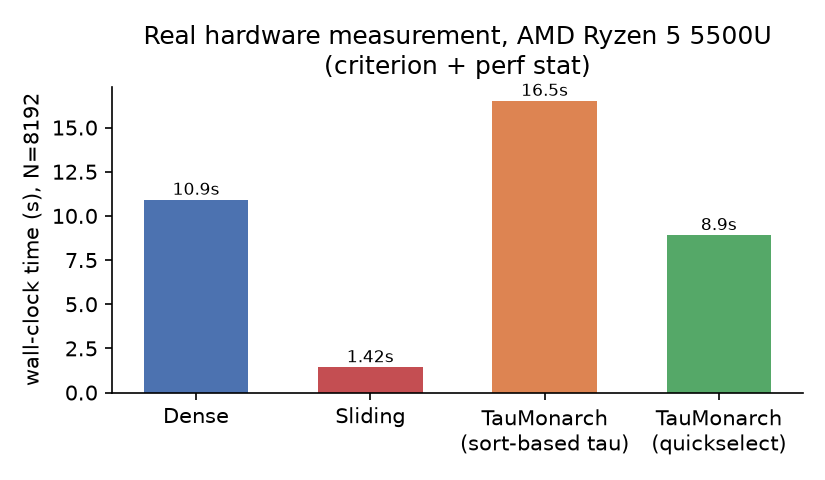
\includegraphics[width=0.6\linewidth]{figures/fig5_hardware_wallclock.png}
\caption{Real hardware wall-clock, $N{=}8192$, AMD Ryzen~5~5500U. The sort-based $\tau$ implementation is slower than dense attention; replacing it with quickselect (mathematically identical $\tau$ value) recovers a genuine 1.22$\times$ win.}
\end{figure}

Confirming this held on the real production model configuration (grouped-query attention,
head\_dim=64, n\_q\_heads=14, n\_kv\_heads=2), a roofline analysis placed both dense attention
and TauMonarchAttention decisively in the compute-bound regime---but with materially
different margins, which we report separately rather than merged, after an earlier draft
of this same analysis was caught conflating the two: TauMonarchAttention lands
$\sim$15--28$\times$ above the 5500U's estimated memory/compute ridge point at the
project's target sequence lengths, while dense attention, doing strictly more total work,
lands further above it still, $\sim$25--48$\times$. Both margins are wide enough that
neither conclusion depends on optimistic assumptions about kernel efficiency, and both
mechanisms' realized FLOP reduction should, and did, translate into wall-clock time rather
than being absorbed by memory bandwidth.

\begin{figure}[htbp]
\centering
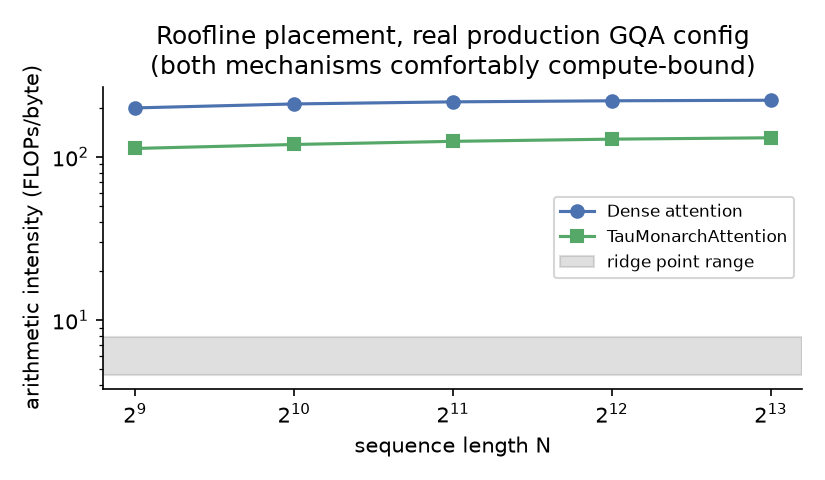
\includegraphics[width=0.62\linewidth]{figures/fig10_roofline_ridge_point.png}
\caption{Implied arithmetic intensity of dense attention and TauMonarchAttention at the real production GQA configuration, against the 5500U's estimated compute/memory ridge point. Both mechanisms sit well above the ridge across the project's target sequence lengths.}
\end{figure}

\section{Trained Landmark Selection: A Closed Question}

Every mechanism in Sections~4.1--4.6 used an \emph{untrained}
representative-construction heuristic. Gradient-trained representative construction had
never been tested in this investigation and was flagged as the one genuinely open axis:
real published landmark-attention systems use trained, not untrained, summarizers, which
is suggestive but not dispositive.

\subsection{Architecture and objective}

A small trainable module (a per-key MLP transform followed by multi-head attention
pooling) was trained to select, not summarize: given real per-key scores against a
query, decide which block to route real attention to. Two training regimes were compared:
an indirect retrieval loss (maximize cosine similarity to the true value) and a direct
listwise cross-entropy loss on block-selection scores. Both regimes produced statistically
indistinguishable selection accuracy (37.1\% vs.\ 34.7\% at $M{=}16$ candidate blocks,
3-seed spread 3.0 percentage points)---ruling out training-objective mismatch as the
bottleneck. The mean selection margin (needle's own score minus the best competing
block's score) was \emph{negative} at every seed tested, and a sweep across candidate-block
count $M$ confirmed an order-statistic explanation: margin degrades smoothly as
$\sqrt{2\ln M}$, a structural property of extreme-value competition, not an
artifact of training procedure.

\begin{figure}[htbp]
\centering
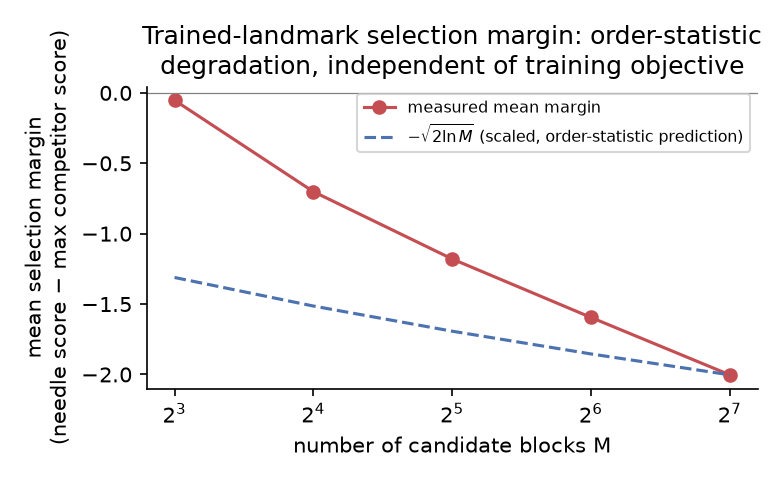
\includegraphics[width=0.62\linewidth]{figures/fig12_landmark_margin_sweep.png}
\caption{Mean selection margin (the trained landmark's needle score minus its best competitor's score) falls smoothly with candidate-block count $M$, closely tracking the theoretical $-\sqrt{2\ln M}$ order-statistic prediction (dashed, scaled for shape comparison)---a structural ceiling, not a training artifact.}
\end{figure}

\subsection{The pre-committed kill criterion, and a bug in our own first attempt}

Per Section~3.3's discipline, a numerical bar was fixed before running the deciding
experiment: recovering $\geq$80\% of TauMonarchAttention's retrieval quality must not require
admitting more than 50\% of candidate blocks to real scoring. A first implementation, using
a fixed top-$k$ admission quota, passed this bar comfortably (30\% admission recovered 84.5\%
of reference quality). This result was itself an artifact: a fixed quota always admits
exactly $k$ blocks regardless of the landmark's actual confidence, an implicit guarantee
genuine Louver-style thresholding does not provide. Replacing the quota with a real,
score-based threshold---and catching a second bug in our own first attempt at this
replacement, where a per-query quantile of that same query's own scores was found to
silently reproduce the same rank-based guarantee (zero variance in admitted-block-count
across 30 trials, a tell that immediately exposed the error)---produced a materially
different result once corrected with a genuinely query-independent threshold: the
80\%-quality target was only reached at 61.7\% average block admission, failing the
pre-committed 50\% cap.

\begin{figure}[htbp]
\centering
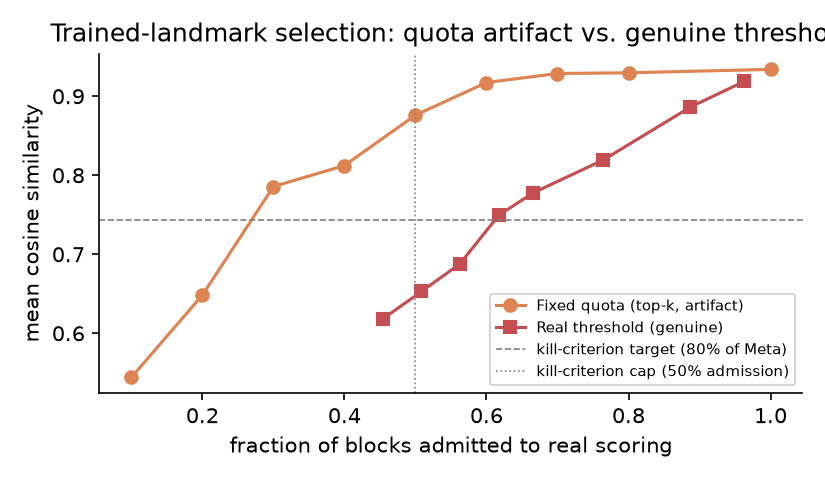
\includegraphics[width=0.62\linewidth]{figures/fig6_landmark_kill_criterion.png}
\caption{The fixed-quota admission scheme clears the pre-committed kill criterion easily; the genuine, query-independent threshold does not---the 80\%-quality target is only reached past the 50\% admission cap.}
\end{figure}

\subsection{Economics, independent of the accuracy result}

A separate FLOP accounting of the trained landmark's per-key construction cost found it to
be 72$\times$ a real per-key dot product (verified by direct computation, dimension-independent).
Amortizing this cost across all future queries that reuse a cached, once-computed
representative (architecturally analogous to TauMonarchAttention's own precomputed
block sums) would have made the 30\%-admission (quota) result genuinely economical relative
to TauMonarchAttention's own scoring cost---but this amortization assumption was never
tested, and the accuracy result in Section~8.2 makes it moot: the real
admission rate required is 61.7\%, not 30\%, at which point the mechanism offers no
meaningful advantage over simply reading everything.

\subsection{Verdict}

The trained-landmark axis is closed for the architecture and training setup tested. Two
independent lines of evidence---the negative selection margin under direct margin
training, and the real-threshold admission-rate failure---converge on the same
conclusion via different mechanisms, which we regard as stronger grounds for closure than
either alone. Larger-dimension trained landmarks remain a genuinely open, unexplored
question (the tested configuration used a toy head dimension of 16); we do not pursue this
further here, consistent with the proportionate-scope discipline that motivated
pre-committing the kill criterion in the first place.

\section{Discussion}

Every failed mechanism in this report shares a single structural property: it decides what
matters via some compressed, pre-score summary of a block's content---a centroid, a
magnitude statistic, a farthest-point sample, a Sinkhorn-refined representative, a hash
bucket, or a gradient-trained pooling vector. Every one of these, independently and by
different specific mechanics, failed the same adversarial control once that control was
applied. TauMonarchAttention's defining property is not any particular architectural
cleverness; it is the absence of this failure mode by construction---survivorship is
always decided by a key's own real score, and the one place compression is still used (the
non-survivor aggregate) only ever aggregates content that has already lost the real-score
comparison, never content that might have been the answer.

A second, methodological thread runs through this report, and it is more frequent than a
short list can convey: repeated instances where an analytically or synthetically favorable
result was reversed only after real measurement. The most consequential examples are
detailed in this paper---the residual-centroid FLOP omission (Section~7.2), the
sort-cost discovery on real hardware (Section~7.3), and the fixed-quota artifact in
the trained-landmark kill criterion (Section~8.2)---but the underlying research log
records a longer tail of the same pattern at smaller scale: a scaling-factor
(head-count) bug and a missing grouped-query-attention correction in an early roofline
calculation, a tiling-convention mismatch in a memory-traffic comparison, and a
cost-model table row that asserted a cheap threshold-estimation method had been built and
measured when it had, at that point, only been proposed. We report the three headline
cases in detail because they are the ones that changed a design or cost conclusion; we
name the smaller ones here explicitly rather than let their absence imply this was a rare
occurrence. In every case, the discipline that caught the error was the same: treat a
plausible-sounding result as a hypothesis to be checked against a harder, more
adversarial, or more directly-measured version of the same question, not as a conclusion.
We think this discipline, more than any single design choice, is the transferable
contribution of this report.

\section{Conclusion}

TauMonarchAttention---Fenwick-tiered shared-threshold selection over real per-key
scores, with an exact-algebraic non-survivor aggregate, quickselect-based threshold
estimation, and no iterative refinement---is, to our knowledge, the only mechanism in
this eight-way comparison that survives a same-norm-controlled adversarial needle probe
at parity with dense attention itself. On the target hardware, it delivers a real,
hardware-measured 1.22$\times$ wall-clock speedup over dense causal attention at the
project's target context lengths. Every alternative we tested that relies on a compressed
representative computed before real per-key scoring---whether hand-designed, iteratively
refined, or gradient-trained---failed the same control. We regard the eight-mechanism
negative-result arc, and the specific discipline that produced it (same-norm adversarial
construction, multi-seed statistics, pre-committed kill criteria, and hardware-measured
rather than analytical cost claims), as the report's primary contribution, with
TauMonarchAttention itself as its validated output.

\begin{thebibliography}{9}

\bibitem{louver}
``Sparse Attention as a Range Searching Problem: Towards an Inference-Efficient Index
for KV Cache.'' arXiv:2605.06763, 2026. Reformulates sparse attention as halfspace range
searching; an index structure guaranteeing zero false negatives with respect to a
specified threshold.

\bibitem{landmark}
A.~Mohtashami and M.~Jaggi. ``Landmark Attention: Random-Access Infinite
Context Length for Transformers.'' arXiv:2305.16300, 2023. NeurIPS 2023. Trains a landmark
token per block to select relevant blocks for retrieval within the attention mechanism.

\bibitem{monarch}
T.~Dao, B.~Chen, N.~Sohoni, A.~Desai, M.~Poli, J.~Grogan, A.~Liu, A.~Rao, A.~Rudra,
C.~R\'e. ``Monarch: Expressive Structured Matrices for Efficient and Accurate Training.''
arXiv:2204.00595, 2022. ICML 2022 (PMLR~162). Block-diagonal butterfly-factorized
structured matrices for hardware-efficient training.

\bibitem{monarchattn}
C.~Yaras, A.~S.~Xu, P.~Abillama, C.~Lee, L.~Balzano. ``MonarchAttention:
Zero-Shot Conversion to Fast, Hardware-Aware Structured Attention.'' arXiv:2505.18698, 2025.
Computes an optimization-based approximate projection of an already-trained, non-causal
dense softmax attention layer onto the class of Monarch matrices, with no additional
training; reports 1.4--8.2$\times$ wall-clock speedup over FlashAttention-2. The
originating work this investigation adapts to the causal, from-scratch-trained setting
(Section~2.1).

\bibitem{moba}
E.~Lu et al.\ (Moonshot AI). ``MoBA: Mixture of Block Attention for Long-Context LLMs.''
arXiv:2502.13189, 2025. Applies mixture-of-experts routing principles to block-sparse
attention, deployed in production for long-context inference.

\end{thebibliography}

\end{document}
